\chapter{Experiment}

\section{Goal of the Experiment}
The main purpose of the experiment is to show that Reinforcement Learning from visual input is possible using Vizia Environment. 	
Additionally, the eperiment tries to investigate how skipping varying number of frames influences learning process.

\section{Experiment's Design}
During the experiment agents with varying \emph{skiprates} are to be tested. We define \emph{skiprate} as the number of game frames that are skipped(ignored) by agent for every frame that is processed. Skipping a frame is acomplished with makeAction method with tics argument set to skiprate (see TODO /REF/) so rewards are acummulated and the chosen action is extended for the duration of skipped frames. Skiprate values of 0,1,2,3,4,5~and~7 are included in the experiment. 

Every agent is to run 80 epochs. Each epoch requires performing 5000 learning steps that involve performing an action (observing transition) and running a learning update. After the learning portion of each epoch, 100 random test episodes are conducted and mean score is used for assessment.  

\section{Tested Agent's Design}
	The agent is heavily inspired by Google DeepMind Atari DQN \cite{mnih-dqn-2015}\cite{mnih-atari-2013} and is conceptually identical to the aformentioned algorithm. Game is modelled as a Markov Decision Process and Q-learning\cite{watkins:mlj92} is used to reach the optimal policy. $\epsilon$-greedy policy with linear $\epsilon$ decay is used to choose actions. Additionally, a technique called experience replay\cite{mnih-dqn-2015} is applied. State is represented by only the most recent image therefore agents have no memory. A convolutional Neural Network is used for approximation of q-values and it is trained with Backpropagation Algorithm\cite{lecun-98b} using Stochastic Gradient Descent with mini-batches. Agent is written in Python and uses Theano\cite{Bastien-Theano-2012}\cite{bergstra+al:2010-scipy} and Lasagne\cite{sander_dieleman_2015_27878} to implement neural networks. Neural network's forward and backword passes were computed using a GPU whereas the rest of the code run on the CPU.

\newpage
\section{Experimental Setup} 
	\subsection{Operating System and Hardware}
	\begin{description}
		\item[Operating System] Linux Mint 17 x86\_64, kernel 3.13.0-24-generic
		\item[CPU] Intel Core i7-4790, 4x4GHz
		\item[GPU] GeForce GTX 970, 1664 CUDA cores, 4GB RAM
	\end{description}

	\subsection{Game Settings}
		The experiment uses the simplest scenario from the pool, that is the `basic' scenario (see \ref{subsec:basic}). State is represented by 3-channel image (RGB) with resolution of 60 by 45 pixels.

	\subsection{Neural Network Architecture}
		\begin{figure}
			\centering
			
\includegraphics[scale=0.4]{network.jpg}
			\caption{Schematic illustration of neural network used for the experiment.}\label{fig:network}
		\end{figure}
		 Used network consists of two convolutional layers with 32 square filters (7 and 4 pixels wide) each connected to a max-pooling layer with poolsize equal to 2 and rectifiers. Convolutional layers are followed by a fully connected layer with 800 leaky rectified linear units and output layer with 8 linear units coresponding to 8 available actions (combinations of 3 available buttons). The architecture used is rather a modest one, nonetheless it still might be excesively robust for such a simple problem.
	
	\subsection{Hyper Parameters}
		\begin{itemize}
		\item $\gamma$ (discount factor) = 0.99
		\item learning rate = 0.01
		\item mini-batch size = 40
		\item initial $\epsilon$ = 1.0
		\item final $\epsilon$ = 0.1
		\item steps after which $\epsilon$ decay will start = 100000
		\item steps to fully decrease $\epsilon$ = 100000
		\item replay memory  capacity = 10000
		\end{itemize}
	

\section{Results}
	\subsection{Numerical Issues}
		In case of 0 skiprate a major numerical problem was euncountered. Estimated q-values usually ($\approx$50\% of runs) rapidly grew to infinite vallues (in the first epoch) which prevented further learning. Quite unexpectedly, increasing resolution from 60x45 to 120x90 eliminated the problem at the cost of longer learning time. Faulty code would be an obvious explenation, however no apparent error has been found yet therefore a conceptually oriented mechanism is also be considered. It is suggested that combination of zero skiprate and low resolution may produce state transitions that incorporate barely distinguishible states. As a consequence each update would signifficantly infalte q-values for each state and rapidly reach infinity. Although changing the resolution seems to have solved the problem, it is not a satisfying solution and one based on theory of q-learning would be much more desirable.

		Skiprate 0 setting was tested for both resolutions, however the agent with increased resolution is considered separately (see Figure \ref{fig:results_skiprate0}).Due to high number of epochs required to get fairly satisfying results with zero skiprate and increased resolution, learning was continued for further 270 epochs to see if it would follow the trend as expected.

	\subsection{Learning Quality}
		As seen in the Figure \ref{fig:results} all agents reached estimated maximum average score of ~80 or showed trend towards achieving similar value. Watching agents play the scenario proved that agents in fact behave very reasonably. They move towards the target and shoot when it appears in front of them. Occasionally agents fire marginally too soon or stay idle (first available action) throughout whole episode. 

	\subsection{Skiprate Influence}
		
		\subsubsection*{Learning speed} 
			\begin{table}
				\begin{center}
					\begin{tabular}{ |l | c |}
						\hline
						Skiprate & Average epoch duration [s] \\ \hline
						0 & 51.79 \\ \hline
						1 & 51.83 \\ \hline
						2 & 52.84 \\ \hline
						3 & 53.84 \\ \hline
						4 & 52.88 \\ \hline
						5 & 53.15 \\ \hline
						7 & 53.12 \\ \hline
					\end{tabular}
				\end{center}
				\caption{Influence of skiprate on processing time for resolution of 60X45}\label{tab:time_results}
			\end{table}
			As seen in the Figure \ref{fig:results} higher skiprate leads to quicker (in terms of learning steps) and smoother learning, which was expected as higher skiprate makes consequences of actions more immediate and easier to notice. However, it must be pointed out that epoch's duration slightly increases with raising skiprate (see Table \ref{tab:time_results}). Obiously, such behavior was anticipiated because Doom engine has to process skiprate as many frames for a single state snapshot.

		\subsubsection*{Score}
			\begin{table}
				\begin{center}
					\begin{tabular}{ |l || c | r |}
						\hline
						Skiprate & Best epoch score & Mean of 10 best epochs \\ \hline
						0 & 69.18 & 60.973 \\ \hline
						1 & 77.84 & 76.187 \\ \hline
						2 & 79.35 & 77.914 \\ \hline
						3 & 80.98 & 78.695 \\ \hline
						4 & 81.8 & 80.755 \\ \hline
						5 & 81.32 & 80.162 \\ \hline
						7 & 81.08 & 80.496 \\ \hline
					\end{tabular}
				\end{center}
				\caption{Influence of skiprate highscores achieved in 80 epochs.}\label{tab:results}
			\end{table}
			It was also anticipated that higher skiprate would slightly lower scores due to the lack of small-grained control. As seen in Table \ref{tab:results}, just the oposite seems to be true. It is doubtful that too short training is the culprit since most of agents reach signifficant stability in 80 epochs and do not appear to be able to ever transcend achieved highscores (at least for skiprates $\geq$ 2). What is more, it was observed that agents with higher skiprates were less prone to irrational behaviours like staying idle or going the oposite way which may coincide with much smoother learning. However, it is suggested that careful fine-tuning of hyper parameters could positively influence learning rate and smoothness. 

			Learning process was especially fuzzy for zero skiprate with increased resolution (see Figure \ref{fig:results_skiprate0}) but it appears that it was slowly converging to the optimum and intensity of ocassional terrible-performance episodes was fading. Further learning (preferably with lowered learning rate) would be neccessary to confirm the hypothesis.
	
	\begin{figure}
		\centering
		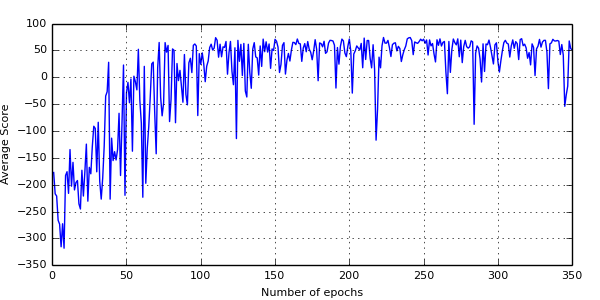
\includegraphics{results_skiprate0.png}
		\caption{Graphs showing mean performance of agent with zero skiprate and resolution 120x90 throughout 350 learning epochs.}\label{fig:results_skiprate0}
	\end{figure}

	\begin{figure}
		\centering
		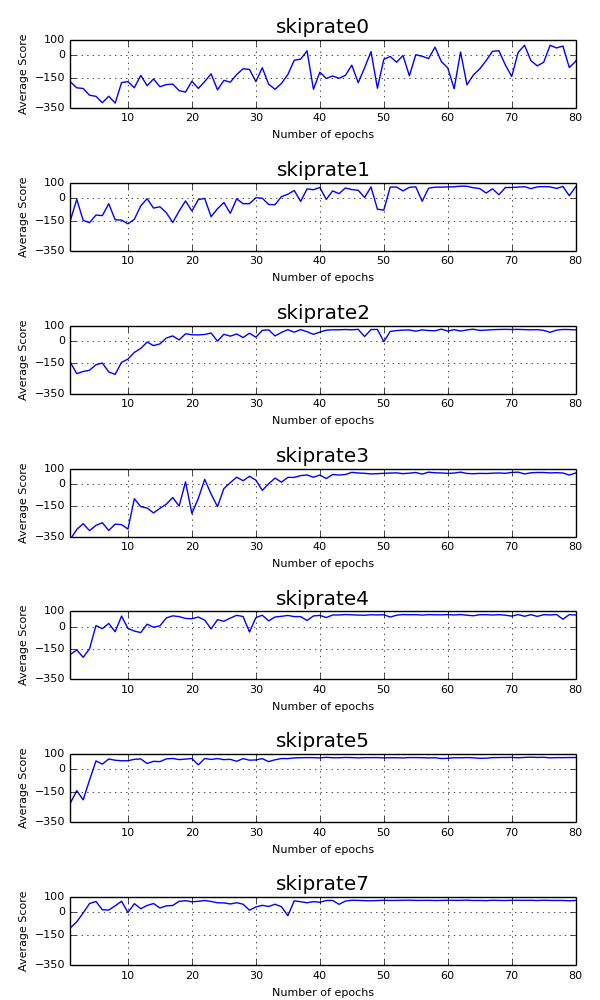
\includegraphics{results.png}
		\caption{Graphs showing mean performance of tested agent with different skip values throughout 80 learning epochs.}\label{fig:results}
	\end{figure}